\chapter[Создание элементов графического интерфейса]{Собственные классы в Qt.
Создание элементов графического интерфейса}
\section[Класс QObject]{Класс QObject}
\index{Класс!QObject}\Sys{QObject} является базовым классом для почти всех классов \Sys{Qt}. Исключением являются только
классы, которые должны быть достаточно <<легкими>> (экземпляры которых должны занимать как можно меньше
памяти) и классы, объекты которых должны копироваться (\Sys{QObject} не поддерживает копирования), а также
контейнерные классы. Все виджеты \Sys{Qt} наследуют \Sys{QObject} (класс \Sys{QWidget} является потомком
\Sys{QObject}). \Sys{QObject} реализует все базовые особенности, которыми обладают классы \Sys{Qt}:

\begin{itemize}
\item мощный механизм взаимодействия между объектами с помощью сигнально-слотовых соединений;
\item иерархические взаимосвязи между объектами, позволяющие объединять их в объектные деревья;
\item управление памятью;
\item «умные» указатели, позволяющие отслеживать уничтожение объекта;
\item поддержка свойств;
\item таймеры;
\item обработка событий и фильтры событий;
\item метаинформация о типе объекта, его свойства и т. п.
\end{itemize}
Каждый объект типа \Sys{QObject} обладает метаданными, которые хранятся внутри специального
\index{Метаобъект}метаобъекта. Этот метаобъект создается для каждого потомка \Sys{QObject} и сохраняет
различную информацию об объекте (так называемые метаданные). Среди доступных для программиста метаданных есть:

\begin{itemize}
\item имя класса (метод \Sys{const chat *Qobject::className()});
\item наследование (метод \Sys{bool QObject::inherits(const char *className)});
\item информация о свойствах;
\item информация о сигналах и слотах;
\item общая информация о классе (\Sys{QОbject::classInfo}).
\end{itemize}
Метаданные собираются во время компиляции (предварительной обработки проекта с помощью \Sys{qmake})
метаобъектным компилятором \Sys{moc}, который анализирует содержание заголовочных файлов программы. Эти метаданные
позволяют получить информацию про любого потомка \Sys{QObject}. Эта информация может быть полезна как для отладки
программы, так и для создания различных механизмов взаимодействия между объектами в программе.

При разработке с использованием \Sys{Qt} часто возникает необходимость наследовать класс \Sys{QObject} непосредственно или
его потомка. Объекты, которые наследуют \Sys{QObject}:

\begin{itemize}
\item объекты имеющие имя (\Sys{QObject :: objectName ()}), которое используется в \Sys{Qt} для реализации различных
возможностей (стили, \Sys{QML} и т.д.);
\item объекты, которые могут занимать место в иерархии других объектов \Sys{QObject};
\item объекты, которые могут иметь сигнально-слотовые соединения с другими \Sys{QObject}.
\end{itemize}

Рассмотрим создание собственного класса на примере создания виждета, который можно будет многократно использовать в
разных программах. Разработаем поле ввода с пиктограммой, которая может реагировать на действия пользователя. Такая
пиктограмма:

\begin{itemize}
\item может быть статически изображена в поле ввода (например, для обозначения обязательных полей в форме ввода данных
пользователем);
\item обозначать пустое поле или поле с введенными данными (например, для обозначения некорректно введенных данных);
\item выполнять заранее заданное действие после нажатия (например, для открытия диалога выбора файла для поля ввода пути
к файлу).
\end{itemize}

Создадим новый проект и добавим к нему новый класс, который будет наследовать от \Sys{QLineEdit} (создание новых
классов с использованием мастера описано в разделе~\ref{ch13:1}). Назовем новый класс \Sys{IconizedLineEdit}. После создания
нового класса откроем файл описания (\Sys{IconizedLineEdit.h}).

Для того, чтобы корректно наследовать класс от \Sys{QObject} необходимо выполнить несколько условий:

\begin{itemize}
\item во-первых, \Sys{QObject} (или потомок \Sys{QObject}, от которого наследуют) должен стоять первым в списке
классов, от которых наследуют;
\item во-вторых, перед объявлением интерфейса класса сразу после фигурной скобки в частной секции размещают макрос
\Sys{Q\_OBJECT}. 
\end{itemize}
Созданный класс выполняет эти условия (наследует от \Sys{QLineEdit}, который наследует от \Sys{QWidget}, а тот в
свою очередь от \Sys{QObject} и содержит макрос \Sys{Q\_OBJECT} в частной секции класса).
\begin{lstlisting}
#ifndef QRCLEARABLELINEEDIT_H
#define QRCLEARABLELINEEDIT_H
#include <QLineEdit>
class QLabel;
class IconizedLineEdit : public QLineEdit
{
  Q_OBJECT
public:
  //`Режимы отображения пиктограммы, которые определяют ее поведение`
  enum IconVisibilityMode {
    //`Всегда отображать пиктограмму`
    IconAlwaysVisible =0,
    //`Отображать пиктограмму после наведения курсора на поле ввода`
    IconVisibleOnHover,
    //`Отображать пиктограмму при присутствии текста`
    IconVisibleOnTextPresence,
    //`Отображать пиктограмму при отсутствии текста`
    IconVisibleOnEmptyText,
    //`Всегда прятать пиктограмму`
    IconAlwaysHidden
    };
    explicit IconizedLineEdit(QWidget *parent = 0);
    bool isIconVisible() const;
    void setIconPixmap(const QPixmap &pPixmap);
    void setIconTooltip(const QString &pToolTip);
private:
    void updateIconPositionAndSize();
private:
    QLabel *mIconLabel; //`Указатель на метку, которая отображает пиктограмму`
};
#endif // QRCLEARABLELINEEDIT_H
\end{lstlisting}


В конструкторе класса создадим метку \Sys{mIconLabel} с помощью которой мы будем отображать значок. Также добавим
реализацию для нескольких вспомогательных методов.
\begin{lstlisting}
#include "iconizedlineedit.h"
#include <QStyle>
#include <QLabel>
//`Конструктор класса`
IconizedLineEdit::IconizedLineEdit(QWidget *parent) : QLineEdit(parent)
{
  mIconLabel = new QLabel(this); //`Создаем метку для того, чтобы показать пиктограмму`
}
//`Возвращает true, если пиктограмма видима`
bool IconizedLineEdit::isIconVisible() const
{
    return mIconLabel->isVisible();
}
//`Устанавливает пиктограмму`
void IconizedLineEdit::setIconPixmap(const QPixmap &pPixmap)
{
  //`Устанавливаем пиктограмму для метки`
  mIconLabel->setPixmap(pPixmap);
  //`Обновляем позицию и размеры`
  updateIconPositionAndSize();
}
//`Устанавливаем подсказку для пиктограммы`
void IconizedLineEdit::setIconTooltip(const QString &pToolTip)
{
  //`Подсказка будет видимой после наведения курсора на метку с пиктограммой`
  mIconLabel->setToolTip(pToolTip);
}
void IconizedLineEdit::updateIconPositionAndSize()
{
  //`Обновить размер пиктограммы`
  mIconLabel->setScaledContents(true);
  mIconLabel->setFixedSize(height(), height());
  //`Обновить размещение пиктограммы`
  QSize lSize = mIconLabel->size();
  mIconLabel->move(rect().right() - lSize.width(),(rect().bottom() + 1 - lSize.height())/2);
}
\end{lstlisting}

Чтобы показать значок, мы используем метку, изображения для которой можно передать с помощью метода
\Sys{setPixmap()}. Этот метод принимает экземпляр \index{Класс!QPixmap}\Sys{QPixmap} класса для работы с
растровыми изображениями.

Метод \Sys{updateIconPositionAndSize()} обновляет размер и размещение для метки. Для того, чтобы
растянуть{\textbackslash}сжать изображения мы передаем \Sys{true} методу метки\Sys{ setScaledContents}(). Это
позволяет игнорировать размеры изображения и изменить размер для значков. Далее мы устанавливаем фиксированный размер
для метки, таким образом, чтобы ее пропорции подходили для размещения в поле. Затем размещаем метку в правом конце
текстового поля.

Для того, чтобы установить тот или иной режим отображения значка запрограммируем метод \Sys{setIconVisibility()}.
Добавим объявление метода в файл описания, а также добавим описание перечисления \Sys{IconVisibilityMode},
содержащее режимы отображения пиктограммы.
\begin{lstlisting}
public:
  //`Режимы отображения пиктограммы, которые определяют ее поведение`
  enum IconVisibilityMode 
  {
    //`Всегда отображать пиктограмму`
    IconAlwaysVisible =0,
    //`Отображать пиктограмму после наведения на поле ввода`
    IconVisibleOnHover,
    //`Отображать пиктограмму при присутствии текста`
    IconVisibleOnTextPresence,
    //`Отображать пиктограмму при отсутствии текста`
    IconVisibleOnEmptyText,
    //`Всегда прятать пиктограмму`
    IconAlwaysHidden
  };
void setIconVisibility(IconVisibilityMode pIconVisibilityMode);
....
private slots:
  void slotTextChanged(const QString &pText);
private:
  void updateIconPositionAndSize();
  void setIconVisible(bool pIsVisible);
private:
  IconVisibilityMode mIconVisibilityMode; //`Режим отображения`
\end{lstlisting}

Для того, чтобы слот \Sys{slotTextChanged(QString)} работал, добавим в конструктор сигнально-слотовое соединение.
Также добавим начальную инициализацию для поля \Sys{mIconVisibilityMode}.
\begin{lstlisting}
//`Конструктор класса`
IconizedLineEdit::IconizedLineEdit(QWidget *parent) : QLineEdit(parent), mIconVisibilityMode(IconAlwaysVisible) //`Инициализация`
{
  mIconLabel = new QLabel(this); //`Создаем метку для того, чтобы показать пиктограмму`
  //`Обработка изменения текста в поле`
  connect(this, SIGNAL(textChanged(QString)),this,SLOT(slotTextChanged(QString)), Qt::UniqueConnection);
}
\end{lstlisting}

Чтобы использовать наш виджет в программе, добавим файл описания класса и создадим несколько экземпляров, которые
разместим на форме. Ответственным за создание интерфейса окна будет отдельный метод \Sys{createUi()}.

В файле описания класса главного окна напишем:
\begin{lstlisting} 
#include <QWidget>
class IconizedLineEdit;
class MainWindow : public QWidget
{
  Q_OBJECT
public:
  explicit MainWindow(QWidget *parent = 0);
private:
  void createUi();
private:
  IconizedLineEdit *iconizedLineEdit;
  IconizedLineEdit *iconizedLineEdit_2;
  IconizedLineEdit *iconizedLineEdit_3;
  IconizedLineEdit *iconizedLineEdit_4;
  IconizedLineEdit *iconizedLineEdit_5;
};
\end{lstlisting}


В файле реализации главного окна разместим код:
\begin{lstlisting} 
nclude "mainwindow.h"
#include "iconizedlineedit.h"
#include <QVBoxLayout>
MainWindow::MainWindow(QWidget *parent) :
QWidget(parent)
{
    createUi();
}
void MainWindow::createUi()
{
QVBoxLayout *lMainLayout = new QVBoxLayout;
setLayout(lMainLayout);
iconizedLineEdit = new IconizedLineEdit;
iconizedLineEdit->setPlaceholderText("Click to open file");
iconizedLineEdit->setIconPixmap(QPixmap("Folder.png"));
iconizedLineEdit->setIconVisibility(IconizedLineEdit::IconAlwaysVisible);
lMainLayout->addWidget(iconizedLineEdit);
iconizedLineEdit_2 = new IconizedLineEdit;
iconizedLineEdit_2->setPlaceholderText("Enter IP address");
iconizedLineEdit_2->setIconPixmap(QPixmap("Checkmark.png"));
iconizedLineEdit_2->setIconVisibility(IconizedLineEdit::IconAlwaysVisible);
lMainLayout->addWidget(iconizedLineEdit_2);
iconizedLineEdit_3 = new IconizedLineEdit;
iconizedLineEdit_3->setPlaceholderText("");
iconizedLineEdit_3->setIconPixmap(QPixmap("Questions.png"));
iconizedLineEdit_3->setIconVisibility(IconizedLineEdit::IconVisibleOnTextPresence);
lMainLayout->addWidget(iconizedLineEdit_3);
iconizedLineEdit_4 = new IconizedLineEdit;
iconizedLineEdit_4->setPlaceholderText("Cannot be empty...");
iconizedLineEdit_4->setIconPixmap(QPixmap("Warning.png"));
iconizedLineEdit_4->setIconVisibility(IconizedLineEdit::IconVisibleOnEmptyText);
lMainLayout->addWidget(iconizedLineEdit_4);
iconizedLineEdit_5 = new IconizedLineEdit;
iconizedLineEdit_5->setPlaceholderText("Clearable");
iconizedLineEdit_5->setIconPixmap(QPixmap("X.png"));
iconizedLineEdit_5->setIconVisibility(IconizedLineEdit::IconVisibleOnTextPresence);
lMainLayout->addWidget(iconizedLineEdit_5);
}
\end{lstlisting}

Пути к файлам изображений для значков мы передаем в конструктор \index{Класс!QPixmap}\Sys{QPixmap}. Изображения
должны находиться в текущей папке (папке, в которой расположен файл проекта).

После запуска программы мы увидим главное окно и пять полей с пиктограммами. Нашему виджету еще не хватает нескольких
важных возможностей. Значки не двигаются при изменении размера текстовых полей. Также значок не реагирует на нажатие
мышкой. Совершенствование этого примера, а также дальнейшее изучение свойств объектов и виджетов мы продолжим в
следующих параграфах, посвященных обработке событий.

\section[Управление памятью. Иерархии объектов]{Управление памятью. Иерархии объектов}
Как мы уже знаем, каждый объект может иметь объектов <<родительские>> и <<дочерние>> объекты.
Таким образом объекты организуют в иерархические структуры напоминающие дерево. Каждый из объектов может содержать
дочерние объекты, а также иметь родительский объект. Отношение между объектами можно задать либо воспользовавшись
параметром конструктора (при создании), или же с помощью метода \Sys{QObject::setParent()}. Обычно пользуются первым
способом, \index{Родительский виджет}то есть задают родительский объект при конструировании.
\begin{lstlisting}
//`Задаем  родительский виджет с помощью конструктора`
QLabel *lLabel = new QLabel(lSomeWidget);
  //`Задаем  родительский виджет с помощью метода` QObject::setParent()
  QPushButton *lPushButton = new QPushButton;
  lPushButton->setParent(lSomeWidget);
\end{lstlisting}

Если виджет содержит компоновщики, то и компоновщики и все размещенные в нем виджеты автоматически получат «родителя»
(ведь каждый визуальный элемент наследует от \Sys{QWidget}, а тот в свою очередь наследует от
\index{Класс!QObject}\Sys{QObject}). Объекты также могут менять <<родителя>>, для этого достаточно
вызвать метод \Sys{QObject::setParent (QObject *)} с указателем на другой родительский объект. \index{Объектная
иерархия}Объектную иерархию можно увидеть наглядно, воспользовавшись методом \Sys{dumpObjectTree()} класса
\Sys{QObject}. Он выводит в стандартный поток вывода тип и имя всех дочерних объектов. Зададим имена для объектов
\Sys{lLabel} и \Sys{lPushButton}:
\begin{lstlisting}
lLabel->setObjectName("ChildLabel");
lPushButton->setObjectName("ChildPushButton");
\end{lstlisting}

Если теперь вызвать метод \Sys{dumpObjectTree()} для объекта \Sys{lSomeWidget}, то получим вывод:
\begin{lstlisting}
SomeWidget:: 
  QLabel::ChildLabel 
  QPushButton::ChildPushButton 
\end{lstlisting}

Когда родительский объект удаляют, дочерние объекты тоже будут удалены из памяти перед удалением родительского. То же
самое происходит и при удалении виджетов --- все дочерние виджеты в визуальной иерархии тоже удаляются. Это позволяет
управлять высвобождением памяти в программе.

Управление памятью важно, поскольку неуправляемое выделение памяти приводит к \index{Утечки памяти}\emph{утечке памяти
в программе} --- ситуации, когда программа не освобождает память. Если такое неуправляемое выделение памяти повторяется
периодически, а сама программа выполняется относительно долго, то со временем программа будет занимать все больше места
в оперативной памяти. Наконец, таким образом можно исчерпать всю доступную память, что приведет к аварийному завершению
программы и исчерпания ресурсов операционной системы.

Например, при использовании ключевого слова \Sys{new} память выделяется в \index{Динамически распределяемая
память}динамически распределяемой памяти (так называемой «куче» --- \Sys{heap}). Динамическая память должна быть
освобождена от созданных объектов с помощью ключевого слова \Sys{delete} для того, чтобы избежать утечки памяти
(\Sys{memory leak}). Объекты, созданные в динамически распределяемой памяти могут существовать столько, сколько
необходимо. Динамическая память не будет освобождена автоматически, поэтому программист должен самостоятельно следить
за высвобождением выделенной памяти. Рассмотрим следующий пример:
\begin{lstlisting}
#include <QApplication>
#include <QWidget>
#include <QLabel>
#include <QPushButton>
int main(int argc, char *argv[])
{
  QApplication lApplication(argc, argv);
  //`(1) Память в динамически-распределяемой памяти (heap)`
  QWidget *lSomeWidget = new QWidget(0); //`Окно`
  //`Задаем родительский виджет с помощью конструктора`
  QLabel *lLabel = new QLabel(lSomeWidget);
  //`Задаем родительский виджет с помощью метода` QObject::setParent()
  QPushButton *lPushButton = new QPushButton;
  lPushButton->setParent(lSomeWidget);
  lLabel->setText("Label");
  lLabel->move(10, 10);
  lPushButton->setText("Button");
  lPushButton->move(50, 10);
  //`(1) Память в динамически-распределяемой памяти (heap)
  lSomeWidget->resize(150, 50);
  lSomeWidget->show();
  return lApplication.exec();
}
\end{lstlisting}

Хотя с первого взгляда, программа может показаться корректной (она компилируется и выполняется), в ней есть ошибка,
связанная с некорректным управлением памятью. Для того, чтобы проанализировать использование памяти в программе,
воспользуемся программой \index{Valgrind}\Sys{Valgrind}. Это свободно-распространяемая программа для \Sys{Linux} с открытым кодом.
Среда \Sys{Qt Creator} поддерживает работу с этой программой для анализа использования памяти 
и оптимизации программ на \Sys{Qt}.

Перейдите в режим анализа \Sys{Analyse} (\emph{Анализ}) воспользовавшись кнопкой на панели
переключения режимов работы слева или воспользуйтесь комбинацией клавиш \Sys{Ctrl+6}. Снизу под окном
редактирования появится дополнительная панель. В выпадающем списке выберите \Sys{Valgrind Memory Analyzer} (Анализатор памяти
Valgrind) и запустите процесс анализа (нажмите на кнопку с пиктограммой треугольника на панели или выберите в главном
меню \Sys{Analyze->Valgrind Memory Analyzer} (\emph{Анализ->Анализатор памяти Valgrind}). Начнется анализ работы программы и программа запустится. Затем закройте окно программы. После
завершения работы на панели появится сообщение об утечке памяти (см. рис.~\ref{ch14:refDrawing0}).
\begin{figure}[htb]
\begin{center}
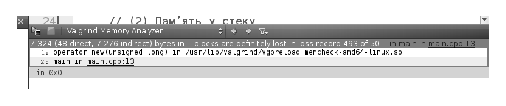
\includegraphics[width=0.8\textwidth]{img/ris_14_1}
\caption[Анализ памяти с помощью Valgrind]{Анализ памяти с помощью Valgrind.}
\label{ch14:refDrawing0}
\end{center}
\end{figure}

Сообщение указывает на строку: 
\begin{lstlisting}
QWidget *lSomeWidget = new QWidget(0); //`Окно`
\end{lstlisting}

Это происходит из-за того, что для \Sys{lSomeWidget} была выделена динамическая память, но не была корректно
высвобождена с помощью оператора \Sys{delete}. Для того, чтобы корректно освободить память, модифицируем последние
строки программы:
\begin{lstlisting}
int exitCode = lApplication.exec();
//`(1) Память в динамически-распределяемой памяти (heap)`
delete lSomeWidget;
return exitCode;
\end{lstlisting}

Скомпилируем программу --- после повторного анализа сообщение об утечке памяти исчезнет. Конечно, в этом примере утечка
памяти не приводит к негативным последствиям. Выделение памяти происходит только раз и после завершения работы вся
использованная оперативная память высвобождается операционной системой. Но в крупных проектах утечки памяти могут стать
серьезной проблемой. Инструменты для анализа памяти такие как Valgrind, позволяют локализовать и исправить их.

Можно выделить память для родительского объекта в стеке. Память для объектов, созданных в стеке, освобождается
автоматически как только объект выходит за пределы области видимости. Поэтому объекты, созданные в стеке, удаляются как
только они выходят из области видимости. Для того, чтобы освободить память автоматически, достаточно только
родительский объект создать в стеке. Как только родительский объект удаляется, будут автоматически удалены и все
дочерние объекты. Мы можем модифицировать последний пример таким образом, чтобы память для родительского объекта была
выделена в стеке. Для этого закомментируйте все части программы обозначенные (1) и измените текст
программы:
\begin{lstlisting}
//`(2) Память в стеке`
SomeWidget lSomeWidget;
//`Задаем родительский виджет с помощью конструктора`
QLabel *lLabel = new QLabel(&lSomeWidget);
//`Задаем родительский виджет с помощью метода` QObject::setParent()
QPushButton *lPushButton = new QPushButton;
lPushButton->setParent(&lSomeWidget);
.....
//`(2) Память в стеке`
lSomeWidget.resize(150, 50);
lSomeWidget.show();
\end{lstlisting}

При описании собственных классов, необходимо помнить следующие рекомендации:

\begin{itemize}
\item задавать для конструкторов класса параметр, который принимает указатель на родительский объект и имеет значение по
умолчанию 0;
\item создавать дополнительный конструктор, который принимает только параметр с указателем на родительский объект;
\item параметр с указателем на <<родителя>> желательно должен быть первым параметром среди параметров со
значением по умолчанию (если параметров со значением по умолчанию несколько);
\item используйте ключевое слово \Sys{this} как указатель на родительский объект при создании объектов внутри своего
класса. Например:
\begin{lstlisting}
#include <QWidget>
class CustomWidget : public QWidget
{
  Q_OBJECT
public:
  explicit CustomWidget(QWidget *parent = 0);
};
//`Конструктор`
CustomWidget::CustomWidget(QWidget *parent) : QWidget(parent)
{
  //`Задаем родительский виджет --- `this `то есть экземпляр класса` CustomWidget
  QPushButton *lPushButton = new QPushButton(this); 
  lPushButton->setGeometry(50, 50, 200, 30);
}
\end{lstlisting}
\end{itemize}

\section[События (Events). Обработка событий (Event handling)]{События (Events). Обработка событий (Event handling)}
В \Sys{Qt} существует механизм, который позволяет обрабатывать различные события, происходящие в системе и в самой программе.
Визуальные элементы пользовательского интерфейса получают события от устройств ввода информации, которыми управляет
пользователь: мышки, клавиатуры и т.п.. Также \index{События}события могут поступать от объектов изнутри приложения.
Таким образом бывают:

\begin{itemize}
\item события, возникшие спонтанно и поступающие от оконной системы, такие как нажатие клавиш, движения мышкой,
манипуляции с окном программы (spontaneous events);
\item события, отправленные изнутри программы, созданные объектами в программе  и направленые в цикл обработки событий
(posted events) или напрямую к другому объекту (sent events).
\end{itemize}
Спонтанные события и большинство внутренних событий поступают в \index{Цикл обработки событий}цикл обработки событий
(\Sys{event loop}). Этот цикл последовательно рассматривает каждое из событий и отправляет на обработку конкретному
объекту. Каждый объект в свою очередь имеет возможность обрабатывать событие, которое поступает к нему.

Каждое событие в \Sys{Qt} существует в виде объекта, унаследованного от \index{Класс!QEvent}\Sys{QEvent}. Когда событие
поступает на обработку, то для объекта-обработчика выполняется виртуальный метод \Sys{QObject::event()}. Этот метод
обычно вызывает другой метод-обработчик события, который для большинства событий является отдельным. Это необходимо для
удобства и гибкости, поскольку таким образом есть возможность запрограммировать обработку конкретного класса событий в
отдельном методе. Почти все основные типы событий реализованы в виде отдельного класса. Например, события для движений
и нажатий клавиш мышки имеют класс \Sys{QMouseEvent}, события для нажатий клавиш клавиатуры имеют класс
\Sys{QKeyEvent} и т. п. В таблице \ref{ch14:refTable0} приведены события, которые часто необходимо обрабатывать при
разработке программ с графическим интерфейсом.

{\tabcolsep=0.3em\noindent\footnotesize
\begin{longtable}{|p{0.2\textwidth}|p{0.4\textwidth}|p{0.35\textwidth}|}
\caption{Часто употребляемые классы событий и их обработчики} \label{ch14:refTable0}\\
\hline
\Emph{Название класса события} &\Emph{Описание} &\Emph{Обработчик события}\\
\hline \hline
\endfirsthead
\multicolumn{3}{c}%
{{\tablename\ \thetable{} --- продолжение}} \\
\hline
\Emph{Название класса события} &\Emph{Описание} &\Emph{Обработчик события}\\
\hline \hline
\endhead
\index{Класс!QMouseEvent}\Sys{QMouseEvent} & Событие для движений мышкой и нажатия клавиш мышки. Посылается виджетам. Выполняется только при нажатии клавиши мышки.
Для того, чтобы виджет постоянно отслеживал этот тип событий, необходимо передать \Sys{true} в метод виджета
\Sys{setMouseTracking()}. &\raggedright
\mbox{клавиша мышки нажата}\linebreak
\lstinline!QWidget::mousePressEvent()!\linebreak
\mbox{клавишу мышки отпустили}\linebreak
\lstinline!QWidget::mouseReleaseEvent()!\linebreak
клавишу мышки нажали два раза\linebreak
\lstinline!QWidget::mouseDoubleClickEvent()!\linebreak 
курсор мышки изменил позицию\linebreak
\lstinline!QWidget::mouseMoveEvent()!
\cr\hline
\index{Класс!QKeyEvent}\Sys{QKeyEvent} &Событие для нажатия клавиш клавиатуры &
\mbox{клавиша нажата}\linebreak
\lstinline!QWidget::keyPressEvent()!\linebreak
\mbox{клавишу отпустили}\linebreak
\lstinline!QWidget::keyReleaseEvent()!
\\\hline
\index{Класс!QResizeEvent}\Sys{QResizeEvent} &Сообщает об изменении размера виджета (изменение уже произошло) &
\lstinline!QWidget::resizeEvent()!
\\\hline
\index{Класс!QPaintEvent}\Sys{QPaintEvent} &Сообщает о необходимости перерисовки виджета &
\lstinline!QWidget::paintEvent()!
\\\hline
\index{Класс!QTimerEvent}\Sys{QTimerEvent} &Посылается через заданные интервалы времени объектом, который запустил один или несколько таймеров с помощью метода \lstinline!QObject::startTimer()!.\linebreak Каждый таймер имеет уникальный идентификатор, который возвращает метод \lstinline!QObject::startTimer()! при создании нового таймера. Таймер можно остановить с помощью вызова метода \lstinline!QObject::killTimer()!. &
\lstinline!QObject::timerEvent()!
\\\hline
\index{Класс!QCloseEvent}\Sys{QCloseEvent} &Посылается окну, которое пользователь пытается закрыть. Позволяет контролировать закрыто окно после обработки события или нет. &
\lstinline!QWidget::closeEvent()!
\\\hline
\end{longtable}
}

Таким образом, для того, чтобы выполнить обработку события, необходимо переопределить нужный обработчик события,
выполнить необходимые для обработки действия и, если необходимо, сохранить стандартное поведение для обработчика ---
вызвать обработчика события из родительского класса. Теперь вернемся к одному из предыдущих примеров --- собственному
виджету для поля ввода с пиктограммой. После изменения размера окна (и поля ввода, которое было размещено в
компоновке), нам необходимо обновить позицию значка для того, чтобы она всегда находилась в правом конце поля ввода.
Для этого мы можем переопределить обработчик события \Sys{QResizeEvent} для класса \Sys{IconizedLineEdit}:
\begin{lstlisting}
//`Событие изменения размера виджета`
void IconizedLineEdit::resizeEvent(QResizeEvent *pEvent)
{
//`Если изменение размера состоялось, обновить позицию и размер пиктограммы`
  updateIconPositionAndSize();
  QWidget::resizeEvent(pEvent);
}
\end{lstlisting}

Для обновления позиции пиктограммы достаточно еще раз вызвать метод
\lstinline!IconizedLineEdit::updateIconPositionAndSize()!. После изменения размера поля ввода позиция пиктограммы будет
автоматически обновлена.

\section[Фильтры событий (Event filters)]{Фильтры событий (Event filters). Распостранение (всплытие) событий (Event propagation)}
Когда цикл обработки посылает событие объекту-адресату, он ожидает, что объект соответствующим образом обработает
событие или сообщит о том, что он не будет выполнять обработку. 
Во втором случае некоторые события могут быть \emph{распостранены} (\EN{propagated}), то есть переданы на обработку к родительскому объекту, если дочерний объект проигнорировал событие.
Примером событий, для которых работает распостранение --- это
события мышки и нажатий клавиш клавиатуры. Они будут <<всплывать>> по обьектной иерархии от дочернего объекта к родительскому, пока один из этих объектов не обработает событие или все не проигнорирует его. 

Для управления этим процессом используют методы \index{Класс!QEvent}\Sys{QEvent::accept()}
(для обозначения события как обработанного) и \Sys{QEvent::ignore()} (для игнорирования события). Их
используют только в виртуальных методах-обработчиках. Обычно \Sys{QEvent::accept()} явно не вызывают,
поскольку большинство распостраняемых событий обозначаются как обработанные по умолчанию.

Несмотря на гибкую систему контроля обработки событий, иногда возникает потребность выполнить обработку вместо
объекта-адресата. Также иногда возникает необходимость заблокировать (отфильтровать) некоторые события, которые
поступают на обработку к объекту. Этого можно достичь с помощью \index{Фильтр событий}\emph{фильтров событий}
(\EN{event filters}).

Фильтры событий являются обычными объектами, унаследованными от \Sys{QObject}. Но перед тем, как событие
поступит к адресату, оно поступает к фильтру событий. Он может передать его дальше на обработку адресату, отсеять или
выполнить необходимые действия в ответ. Для обработки событий, фильтру необходимо переопределить виртуальный метод
\Sys{QObject::eventFilter()}. Этот метод возвращает логическое значение, которое означает, будет ли событие
отфильтровано (значение \Sys{true}) или поступит на дальнейшую обработку (значение \Sys{false}).
Фильтр событий для объекта можно задать с помощью метода \Sys{QObject::installEventFilter()}, который
принимает указатель на \Sys{QObject}, выступающий в роли фильтра. 

Наш предыдущий пример содержит поле ввода с пиктограммой. Для того чтобы реализовать реакцию на нажатие клавиши мыши на
пиктограмму, но не создавать своего класса, унаследованного от класса метки с пиктограммой, мы добавим фильтр событий,
который будет посылать сигнал, если для пиктограммы поступит событие типа \Sys{QEvent::MouseButtonPress}.
Добавим объявление класса \Sys{QEvent}:
\lstinline!#include <QEvent>!

Установим фильтр событий для метки:
\lstinline!mIconLabel->installEventFilter(this);!

И добавим фильтр событий для метки в файле \Sys{IconizedLineEdit.h}:
\begin{lstlisting}
class IconizedLineEdit : public QLineEdit
{
  Q_OBJECT
public:
.....
  void setIconClickable(bool pIsIconClickable);
.....
signals:
  void iconPressed();
protected:
  .....
  bool eventFilter(QObject *pObject, QEvent *pEvent);
.....
private:
.....
  bool mIsIconCklickable;
};
\end{lstlisting}

В файле \Sys{IconizedLineEdit.cpp:}
\begin{lstlisting}
bool IconizedLineEdit::eventFilter(QObject *pObject, QEvent *pEvent)
{
  if (mIsIconCklickable)
  {
    if ((pObject==mIconLabel) && (pEvent->type()== QEvent::MouseButtonPress))
    {
      emit iconPressed();
      return true;
    }
  }
return false;
}
//`Установить режим реакции на нажатие мышкой на пиктограмму`
void IconizedLineEdit::setIconClickable(bool pIsIconClickable)
{
  mIsIconCklickable = pIsIconClickable;
  //`Устанавливаем вид курсора при наведении на метку с пиктограммой`
  if (mIsIconCklickable)
  {
    mIconLabel->setCursor(Qt::PointingHandCursor);
  }
  else
  {
    mIconLabel->setCursor(Qt::ArrowCursor);
  }
}
\end{lstlisting}

Наш класс для поля ввода с пиктограммой одновременно выступает фильтром событий для метки.

Добавим реакцию на нажатие к двум полям в \Sys{mainwindow.cpp}. 
Первое поле будет открывать диалог выбора
файла и записывать путь к файлу. Последнее поле будет стирать свое 
содержимое в ответ на нажатие пиктограммы:
\begin{lstlisting}
#include <QFileDialog>
.....
void MainWindow::createUi()
{
.....
iconizedLineEdit->setIconClickable(true);
connect(iconizedLineEdit, SIGNAL(iconPressed()),this, SLOT(slotChooseFile()), Qt::UniqueConnection);
.....
iconizedLineEdit_5->setIconClickable(true);
connect(iconizedLineEdit_5, SIGNAL(iconPressed()),
iconizedLineEdit_5, SLOT(clear()), Qt::UniqueConnection);
.....
}
void MainWindow::slotChooseFile()
{
QString lFileName = QFileDialog::getOpenFileName(this, "Open file");
iconizedLineEdit->setText(lFileName);
}
\end{lstlisting}

Объявления слота \Sys{slotChooseFile()} добавим к описанию класса главного окна:
\begin{lstlisting}
class MainWindow : public QWidget
{
  Q_OBJECT
......
private slots:
 void slotChooseFile();
......
};
\end{lstlisting}

После этого наш пример окончательно готов (см. рис.~\ref{ch14:refDrawing1}).

\begin{figure}[htb]
\begin{center}
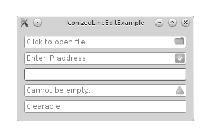
\includegraphics[width=0.5\textwidth]{img/ris_14_2}
\caption[Пример: поле ввода с пиктограммой.]{Пример: поле ввода с пиктограммой.}
\label{ch14:refDrawing1}
\end{center}
\end{figure}

Просуммируем наши знания об обработке событий в \Sys{Qt}:

\begin{itemize}
\item события дают возможность проводить обработку различных ситуаций, возникающих во время работы программы;
\item есть два источника поступления событий. Спонтанные события поступают от оконной системы в ответ на действия
пользователя (движения мышкой, нажатия клавиш клавиатуры, действия с окном программы и т. д.). События также возникают
внутри самой программы и поступают от объектов, которые участвуют в работе программы;
\item события направляются на обработку объектам, участвующим в работе программы. За сбор и перенаправление событий к
обработчикам ответственным является цикл обработки событий в программе;
\item каждое событие существует в виде объекта типа \Sys{QEvent}. Для большинства событий существуют
специализированные классы этих событий, унаследованные от \Sys{QEvent}, которые содержат информацию о событии
и данные необходимые для ее корректной обработки;
\item для участия в обработке событий объект должен быть унаследован от класса \Sys{QObject}. События, которые
поступают к объекту на обработку, автоматически передаются к виртуальному методу
\Sys{QObject::event();}
\item для удобства, для большинства событий существуют отдельные виртуальные методы обработки, которые вызываются
виртуальным методом \Sys{QObject::event();}
\item объекты имеют возможность быть фильтрами событий для других объектов в приложении. Для того, чтобы установить
объект в качестве фильтра событий, пользуются методом \Sys{installEventFilter()}. Объект-фильтр должен
переопределить виртуальный метод \Sys{QObject::eventFilter()}, который возвращает логическое значение, было
событие отфильтровано (то есть, оно не будет направляться на обработку) или нет.
\end{itemize}
А вот общий алгоритм для программной обработки событий:

\begin{itemize}
\item в случае, когда нет возможности унаследовать класс объекта и переопределить методы обработки, а также в случае,
когда необходимо фильтровать, блокировать или предварительно обработать событие перед тем, как она будет отправлена на
обработку к объекту --- воспользуйтесь \index{Фильтр событий}фильтром событий
 \begin{itemize}
 \item переопределите виртуальный метод \Sys{QObject::eventFilter()} для объекта, который будет выступать в
 роли фильтра событий;
 \item в методе \Sys{eventFilter()} проверьте объект к которому на обработку будет направляться событие;
 \item дальше, определите тип события (\Sys{QEvent::Type}) и класс события, проверьте является ли полученное
 событие событием нужного вам типа;
 \item приведите объект события до нужного вам класса событий;
 \item выполните предварительную обработку события, если необходимо. Для того, чтобы отфильтровать событие (после этого
 оно не будет передаваться объекту на обработку) верните из метода логическое значение true. Для того, чтобы отправить
 событие на обработку объекту-адресату верните логическое значение false.
 \end{itemize}

\item для некоторых типов событий, которые не имеют отдельного метода-обработчика, обработку можно запрограммировать,
переопределив метод  \Sys{QObject::event()}
 \begin{itemize}
 \item переопределите виртуальный метод для объекта \Sys{QObject::event()}, который должен выполнять обработку;
 \item определите тип события (\Sys{QEvent::Type}) и класс события, проверьте является  ли полученное событие
 событием нужного вам типа;
 \item приведите объект события до нужного вам класса событий;
 \item выполните обработку или вызовите метод, который ее выполнит, верните значение true, которое означает, что событие
 распознано и обработано, или false в случае, если объект не будет выполнять обработку. В этом случае событие может быть
 переслано на обработку родительскому объекту.
 \item вызовите метод \Sys{event()} для базового класса, чтобы провести обработку всех остальных видов событий.
 Верните из метода значение, которое вернет метод \Sys{event()} базового класса после выполнения.
\end{itemize}

\item если объект имеет виртуальный метод-обработчик события, используйте его
 \begin{itemize}
 \item переопределите виртуальный метод для объекта \Sys{QObject::event()}, который должен выполнять обработку;
 \item выполните обработку события. Вызовите метод \Sys{accept()} для события, если во время обработки
 убедились, что событие должно быть проработано данным объектом. В противном случае, вызовите \Sys{ignore()}
 для объекта события (в этом случае событие может быть направлено к родительскому объекту на обработку).
 \end{itemize}
\end{itemize}

\section[Создание собственного элемента интерфейса]{Создание собственного элемента интерфейса. Создание свойств}
\Sys{QObject} предоставляет механизм для объявления свойств.
\index{Свойства}\emph{Свойства} --- это специальные общедоступные поля, через которые
можно получить доступ к данным объекта. Свойства обычно имеют методы для установки и получения значения, вызываемые при
чтении из свойства и записи данных. В \Sys{Qt} свойства выполняют специальную роль, ведь делают доступными для метаобъектной
системы способы чтения и записи данных объектов, что часто используется в \Sys{Qt} для реализации различных механизмов
(анимации, описание динамических пользовательских интрефейсов в \Sys{QtQuick}, и т.~д.).

Определение свойства обычно состоит из макроса \index{Макрос!Q\_PROPERTY}\Sys{Q\_PROPERTY}, который описывает свойство и содержит описания:
\begin{itemize}
\item метода для установки начального значения;
\item метода для получения значения;
\item метода для установки значения;
\item сигнала об изменении значения свойства;
\item дополнительных настроек.
\end{itemize}

Метод для установки значения принимает одно значение (того же типа, что и свойство) и возвращает \Sys{void}.
Метод для получения значения возвращает значение свойства.

Обычно метод для получения значения называют так же как и свойство, а метод для установки значения еще и имеет префикс
<<\Sys{set}>>. Метод для получения значения, который возвращает тип \Sys{bool} также обычно имеет
префикс <<\Sys{is}>>. например:
\begin{lstlisting}
QStirng text() const;
void setText(const QString &text);
bool isVisible() const;
void setVisible(bool isVisible);
\end{lstlisting}

Наличие отдельного метода для установки значения позволяет запрограммировать 
дополнительные действия, а также проверить
допустимость значения, которое устанавливается. В свою очередь, отдельные 
методы для установки значения дают
возможность косвенного использования уже существующих свойств. 
Изменение значения свойства возможно, как через прямое
использование методов установки и получения значения свойства, так и используя 
средства метаобъектной системы \Sys{Qt}. Также
есть возможность определения доступных свойств во время выполнения программы.

Мы рассмотрим определение свойств на примере создания собственного 
виджета-индикатора \Sys{LedIndicator},
который будет находиться в одном, включенном или выключенном, состоянии 
в зависимости от значения свойства.

Для начала, создадим оконный проект и добавим к нему класс \Sys{LedIndicator}, унаследованный от
\Sys{QWidget}:
\begin{lstlisting}
class LedIndicator : public QWidget
{
  Q_OBJECT
  Q_PROPERTY(QString text READ text WRITE setText)
  Q_PROPERTY(bool turnedOn READ isTurnedOn WRITE setTurnedOn NOTIFY stateToggled)
public:
  explicit LedIndicator(QWidget *parent = 0);
  QString text() const;
  bool isTurnedOn() const;
signals:
  void stateToggled(bool);
public slots:
  void setText(const QString &);
  void setTurnedOn(bool);
private:
  QString mText;
  bool mIsTurnedOn;
};
\end{lstlisting}

Мы определили два свойства: \Sys{text} типа \Sys{QString} для надписи, а также
\Sys{turnedOn} типа \Sys{bool} для состояния индикатора. Специальные слова \Sys{READ} и
\Sys{WRITE} в описании свойства обозначают названия методов для установления и изменения значения свойства. В
описании второго свойства использовано слово \Sys{NOTIFY} для обозначения названия сигнала, который будет
сообщать об изменении свойства. Добавим реализацию для класса:
\begin{lstlisting}
#include <QPainter>
#include <QPaintEvent>
//`Радиус индикатора`
const int cLedRadius = 7;
//`Отступ между индикатором и надписью`
const int cLedSpacing = 5;
LedIndicator::LedIndicator(QWidget *parent) : QWidget(parent),
  mIsTurnedOn(false) //`Инициализируем начальным значением!`
{
}
//`Метод получения значения --- свойство \Sys{text}`
QString LedIndicator::text() const
{
  return mText;
}
//`Метод получения значения --- свойство \Sys{turnedOn}`
bool LedIndicator::isTurnedOn() const
{
  return mIsTurnedOn;
}
//`Метод установки значения --- свойство \Sys{text}`
void LedIndicator::setText(const QString &pText)
{
  mText = pText;
}
//`Метод установки значения --- свойство \Sys{turnedOn}`
void LedIndicator::setTurnedOn(bool pIsTurnedOn)
{
  //`Проверка уже установленного значения`
  if (isTurnedOn() == pIsTurnedOn)
  {
    return;
  }
  mIsTurnedOn = pIsTurnedOn;
  //`Выпускаем сигнал про изменение`
  emit stateToggled(mIsTurnedOn);
  //`Вызываем метод \Sys{QWidget::update()}, который добавляет в очередь событий \Sys{QPaintEvent}`
  //`для того чтобы перерисовать наш виджет в соответствии с установленным \Sys{isTurnedOn()}`
  update();
}
\end{lstlisting}


Обратите внимание: в большинстве случаев при создании собственных \index{Слоты!cоздание}слотов, которые получают и
устанавливают значения, следует сравнивать переданное значение с текущим и запрещать выполнение тела слота, если
переданное и текущее значения равны. Особенно за этим необходимо следить, если слот выдает сигнал об изменении
значения. Об этом необходимо помнить, чтобы избежать бесконечной рекурсии и аварийного завершения программы в случае
перекрестного сигнально-слотового соединения между такими слотами. Именно такую проверку мы выполнили в методе
\Sys{setTurnedOn()} перед отправкой сигнала об изменении и перерисовкой.

Теперь осталось создать для нашего индикатора соответствующий вид. Как мы отметили, существует два способа создать
собственный виджет: составить из готовых виджетов, упорядочив их размещение и геометрию, или нарисовать виджет
средствами \Sys{Qt}. В следующем параграфе мы познакомимся со средствами для прорисовки виджетов на экране.

\section[Рисование элементов. Класс QPainter]{Рисование элементов. Класс QPainter}
Каждый виджет занимает прямоугольную область на экране, в соответствии с позицией и размерами. В пределах этой области
виджет прорисовывает себя когда становится видимым или когда часть этой области была перекрыта или изменилась геометрия
виджета. Для рисования визуальных элементов пользуются примитивами, такими как линии, окружности, прямоугольники,
градиенты и т.~п. Из примитивов складываются сложные элементы, такие как разнообразные рамки, поля, панели и т. д. Для
рисования примитивов в \Sys{Qt} пользуются специальным классом \index{Класс!QPainter}\Sys{QPainter}.

\Sys{QPainter} обладает богатым набором методов для рисования различных геометрических примитивов, надписей и
частей изображений. Для рисования он использует объекты класса \index{Класс!QPaintDevice}\Sys{QPaintDevice},
реализующих область для вывода графической информации (на экран, область памяти, на принтер и т. д.). Класс
\index{Класс!QWidget}\Sys{QWidget} как раз наследует от классов \Sys{QObject} и 
\Sys{QPaintDevice}, что позволяет использовать \Sys{QPainter} для рисования интерфейса.

Оконная система и \Sys{Qt} следят за изменениями размеров, позиции, видимости окон и отдельных виджетов в программе и
направляют специальные события, которые сообщают каждый виджет о необходимости обновления вида. В виртуальном
обработчике \Sys{paintEvent()} виджеты имеют возможность использовать \Sys{QPainter} для
собственного отражения. В нашем примере мы определим обработчик события
\Sys{QPaintEvent}.
\begin{lstlisting}
#include <QWidget>
class LedIndicator : public QWidget
{
  Q_OBJECT
  Q_PROPERTY(QString text READ text WRITE setText)
  Q_PROPERTY(bool turnedOn READ isTurnedOn WRITE setTurnedOn NOTIFY stateToggled)
public:
.....
  QSize minimumSizeHint() const;
....
protected:
  void paintEvent(QPaintEvent *);
.....
};
\end{lstlisting}
И добавим реализацию для него:
\begin{lstlisting}
void LedIndicator::paintEvent(QPaintEvent *pEvent)
{
//`Создаем объект \index{Класс!QPainter}\Sys{QPainter} и указываем \Sys{QPaintDevice} текущий виджет`
QPainter lPainter(this);
//`Используем сглаживание при рисовании для лучшего вида`
lPainter.setRenderHint(QPainter::Antialiasing);
//`Центр окружности индикатора \index{Класс!QPoint}\Sys{QPoint} --- класс для описания точки`
QPoint lLedCenter(cLedRadius + 1, height() / 2);
//`Фигура, которую мы будем рисовать \index{Класс!QPainterPath}\Sys{QPainterPath} --- класс для описания фигуры`
//`состоящей из нескольких примитивов`
QPainterPath lPath;
//`Добавляем окружность`
lPath.addEllipse(lLedCenter, cLedRadius, cLedRadius);
lPainter.save(); //`Сохраняем настройки после всех изменений мы восстановим их для`
//`рисования подписи`
//`Создаем радиальный (окружностями) градиент указываем центр для градиента и радиус`
QRadialGradient lGradient(lLedCenter, cLedRadius);
  if (mIsTurnedOn) //`Устанавливаем цвет границы и градиент`
  {                //`для включенного и выключенного состояний`
  //`Задаем объект \index{Класс!QPen}\Sys{QPen} --- настройки рисования контуров`
  //`Используем константу для задания цвета контура в конструкторе \Sys{QPen}`
    lPainter.setPen(QPen(Qt::darkGreen));
  //`Задаем цвет в разных точках (0 --- центр, 1 --- край) цвет будет равномерно изменяться`
  //`Для задания цвета пользуемся текстовым шестнадцатеричным RGB обозначением`
  //`--- неявное преобразование в \index{Класс!QColor}\Sys{QColor}`
    lGradient.setColorAt(0.2, "#70FF70");
    lGradient.setColorAt(1, "#00CC00");
  }
  else
  {
  //`Здесь задаем черный цвет. Конструктор \Sys{QColor}, значение красной,`
  //`зеленой и синей (0-255) компонент цвета`
    lPainter.setPen(QPen(QColor(0, 0, 0)));
    lGradient.setColorAt(0.2, Qt::gray);
    lGradient.setColorAt(1, Qt::darkGray);
  }
//`Заполняем фигуру индикатора градиентом`
lPainter.fillPath(lPath, QBrush(lGradient));
//`Рисуем границу индикатора`
lPainter.drawPath(lPath);
//`Восстанавливаем настройки перед последним сохранением`
lPainter.restore();
//`Устанавливаем шрифт для рисования текста используем QWidget::font(),` 
//`чтобы иметь возможность стилизовать надпись`
lPainter.setFont(font());
//`Квадрат, в котором будет рисоваться текст. \index{Класс!QRect}\Sys{QRect} --- класс для обозначения прямоуольной области`
QRect lTextRect(cLedRadius*2+cLedSpacing, 0, width()- (cLedRadius*2 + cLedSpacing), height());
//`Рисуем текст в заданном прямоугольнике, выравнивание по левому краю и вертикально по центру`
lPainter.drawText(lTextRect, Qt::AlignVCenter|Qt::AlignLeft, mText);
}
//`Переопределяем виртуальный метод \Sys{minimumSizeHint()} для передачи корректных минимальных размеров\index{Класс!QSize}`
QSize LedIndicator::minimumSizeHint() const
{
  return QSize(cLedRadius * 2   //`Диаметр индикатора`
  + fontMetrics().width(mText)  //`Ширина текста mText`
  + cLedSpacing,                //`Отступ`
  cLedRadius * 2);
}
\end{lstlisting}

Теперь создадим наш виджет и добавим его в главное окно программы вместе с флажком. Соединим флажок и индикатор
сигнально-слотовым соединением, таким образом, что состояние флажка будет ???устанавливаться индикатору.
\begin{lstlisting}
#include <QHBoxLayout>
#include <QCheckBox>
#include "ledindicator.h"
MainWindow::MainWindow(QWidget *parent) : QWidget(parent)
{
//`Главное компонование`
QHBoxLayout *lLayout = new QHBoxLayout;
setLayout(lLayout);
//`Создаем наш индикатор и добавляем его к компоновщику`
LedIndicator *lLedIndicator = new LedIndicator;
lLedIndicator->setText("LED Indicator");
lLayout->addWidget(lLedIndicator);
//`Создаем и добавляем флажок`
QCheckBox *lCheckBox = new QCheckBox("Led ON");
lLayout->addWidget(lCheckBox);
//`Соединяем флажок и индикатор`
connect(lCheckBox, SIGNAL(toggled(bool)),
lLedIndicator, SLOT(setTurnedOn(bool)), Qt::UniqueConnection);
}
\end{lstlisting}

Окончательно, окно нашей программы имеет вид (см. рис.~\ref{ch14:refDrawing2}).

\begin{figure}[htb]
\begin{center}
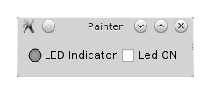
\includegraphics[width=0.3\textwidth]{img/ris_14_3a}\\
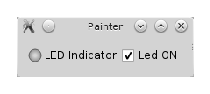
\includegraphics[width=0.3\textwidth]{img/ris_14_3b}
\caption[Пример: виджет-индикатор.]{Пример: виджет-индикатор.}
\label{ch14:refDrawing2}
\end{center}
\end{figure}

\section{Задачи для самостоятельного решения}
\begin{enumerate}
\item Создайте окно для ввода имени пользователя и пароля. Используйте для этого класс \Sys{IconizedLineEdit}.
\item Добавьте возможность проверки правильности введенных данных с помощью класса \Sys{QValidator}. 
\item Создайте программу, которая открывает изображение в окне. Для ввода пути к изображению добавьте к окну поле ввода.
Для поля ввода пути к изображению используйте класс \Sys{IconizedLineEdit}. При нажатии на пиктограмму должен открываться
диалог выбора файла.
\item Добавьте к классу \Sys{LedIndicator} поддержку третьего промежуточного состояния. Для включения поддержки этого
состояния, добавьте метод \Sys{setTristate()}. Для установки и чтения состояния индикатора добавьте методы \Sys{setState}.
\end{enumerate}
